% Options for packages loaded elsewhere
\PassOptionsToPackage{unicode}{hyperref}
\PassOptionsToPackage{hyphens}{url}
\PassOptionsToPackage{dvipsnames,svgnames,x11names}{xcolor}
%
\documentclass[
  letterpaper,
  DIV=11,
  numbers=noendperiod]{scrartcl}

\usepackage{amsmath,amssymb}
\usepackage{iftex}
\ifPDFTeX
  \usepackage[T1]{fontenc}
  \usepackage[utf8]{inputenc}
  \usepackage{textcomp} % provide euro and other symbols
\else % if luatex or xetex
  \usepackage{unicode-math}
  \defaultfontfeatures{Scale=MatchLowercase}
  \defaultfontfeatures[\rmfamily]{Ligatures=TeX,Scale=1}
\fi
\usepackage{lmodern}
\ifPDFTeX\else  
    % xetex/luatex font selection
\fi
% Use upquote if available, for straight quotes in verbatim environments
\IfFileExists{upquote.sty}{\usepackage{upquote}}{}
\IfFileExists{microtype.sty}{% use microtype if available
  \usepackage[]{microtype}
  \UseMicrotypeSet[protrusion]{basicmath} % disable protrusion for tt fonts
}{}
\makeatletter
\@ifundefined{KOMAClassName}{% if non-KOMA class
  \IfFileExists{parskip.sty}{%
    \usepackage{parskip}
  }{% else
    \setlength{\parindent}{0pt}
    \setlength{\parskip}{6pt plus 2pt minus 1pt}}
}{% if KOMA class
  \KOMAoptions{parskip=half}}
\makeatother
\usepackage{xcolor}
\setlength{\emergencystretch}{3em} % prevent overfull lines
\setcounter{secnumdepth}{-\maxdimen} % remove section numbering
% Make \paragraph and \subparagraph free-standing
\makeatletter
\ifx\paragraph\undefined\else
  \let\oldparagraph\paragraph
  \renewcommand{\paragraph}{
    \@ifstar
      \xxxParagraphStar
      \xxxParagraphNoStar
  }
  \newcommand{\xxxParagraphStar}[1]{\oldparagraph*{#1}\mbox{}}
  \newcommand{\xxxParagraphNoStar}[1]{\oldparagraph{#1}\mbox{}}
\fi
\ifx\subparagraph\undefined\else
  \let\oldsubparagraph\subparagraph
  \renewcommand{\subparagraph}{
    \@ifstar
      \xxxSubParagraphStar
      \xxxSubParagraphNoStar
  }
  \newcommand{\xxxSubParagraphStar}[1]{\oldsubparagraph*{#1}\mbox{}}
  \newcommand{\xxxSubParagraphNoStar}[1]{\oldsubparagraph{#1}\mbox{}}
\fi
\makeatother


\providecommand{\tightlist}{%
  \setlength{\itemsep}{0pt}\setlength{\parskip}{0pt}}\usepackage{longtable,booktabs,array}
\usepackage{calc} % for calculating minipage widths
% Correct order of tables after \paragraph or \subparagraph
\usepackage{etoolbox}
\makeatletter
\patchcmd\longtable{\par}{\if@noskipsec\mbox{}\fi\par}{}{}
\makeatother
% Allow footnotes in longtable head/foot
\IfFileExists{footnotehyper.sty}{\usepackage{footnotehyper}}{\usepackage{footnote}}
\makesavenoteenv{longtable}
\usepackage{graphicx}
\makeatletter
\def\maxwidth{\ifdim\Gin@nat@width>\linewidth\linewidth\else\Gin@nat@width\fi}
\def\maxheight{\ifdim\Gin@nat@height>\textheight\textheight\else\Gin@nat@height\fi}
\makeatother
% Scale images if necessary, so that they will not overflow the page
% margins by default, and it is still possible to overwrite the defaults
% using explicit options in \includegraphics[width, height, ...]{}
\setkeys{Gin}{width=\maxwidth,height=\maxheight,keepaspectratio}
% Set default figure placement to htbp
\makeatletter
\def\fps@figure{htbp}
\makeatother

\KOMAoption{captions}{tableheading}
\makeatletter
\@ifpackageloaded{tcolorbox}{}{\usepackage[skins,breakable]{tcolorbox}}
\@ifpackageloaded{fontawesome5}{}{\usepackage{fontawesome5}}
\definecolor{quarto-callout-color}{HTML}{909090}
\definecolor{quarto-callout-note-color}{HTML}{0758E5}
\definecolor{quarto-callout-important-color}{HTML}{CC1914}
\definecolor{quarto-callout-warning-color}{HTML}{EB9113}
\definecolor{quarto-callout-tip-color}{HTML}{00A047}
\definecolor{quarto-callout-caution-color}{HTML}{FC5300}
\definecolor{quarto-callout-color-frame}{HTML}{acacac}
\definecolor{quarto-callout-note-color-frame}{HTML}{4582ec}
\definecolor{quarto-callout-important-color-frame}{HTML}{d9534f}
\definecolor{quarto-callout-warning-color-frame}{HTML}{f0ad4e}
\definecolor{quarto-callout-tip-color-frame}{HTML}{02b875}
\definecolor{quarto-callout-caution-color-frame}{HTML}{fd7e14}
\makeatother
\makeatletter
\@ifpackageloaded{caption}{}{\usepackage{caption}}
\AtBeginDocument{%
\ifdefined\contentsname
  \renewcommand*\contentsname{Table of contents}
\else
  \newcommand\contentsname{Table of contents}
\fi
\ifdefined\listfigurename
  \renewcommand*\listfigurename{List of Figures}
\else
  \newcommand\listfigurename{List of Figures}
\fi
\ifdefined\listtablename
  \renewcommand*\listtablename{List of Tables}
\else
  \newcommand\listtablename{List of Tables}
\fi
\ifdefined\figurename
  \renewcommand*\figurename{Figure}
\else
  \newcommand\figurename{Figure}
\fi
\ifdefined\tablename
  \renewcommand*\tablename{Table}
\else
  \newcommand\tablename{Table}
\fi
}
\@ifpackageloaded{float}{}{\usepackage{float}}
\floatstyle{ruled}
\@ifundefined{c@chapter}{\newfloat{codelisting}{h}{lop}}{\newfloat{codelisting}{h}{lop}[chapter]}
\floatname{codelisting}{Listing}
\newcommand*\listoflistings{\listof{codelisting}{List of Listings}}
\makeatother
\makeatletter
\makeatother
\makeatletter
\@ifpackageloaded{caption}{}{\usepackage{caption}}
\@ifpackageloaded{subcaption}{}{\usepackage{subcaption}}
\makeatother
\ifLuaTeX
  \usepackage{selnolig}  % disable illegal ligatures
\fi
\usepackage{bookmark}

\IfFileExists{xurl.sty}{\usepackage{xurl}}{} % add URL line breaks if available
\urlstyle{same} % disable monospaced font for URLs
\hypersetup{
  pdftitle={MATH 246 - Intermediate Statistics},
  colorlinks=true,
  linkcolor={blue},
  filecolor={Maroon},
  citecolor={Blue},
  urlcolor={Blue},
  pdfcreator={LaTeX via pandoc}}

\title{MATH 246 - Intermediate Statistics}
\usepackage{etoolbox}
\makeatletter
\providecommand{\subtitle}[1]{% add subtitle to \maketitle
  \apptocmd{\@title}{\par {\large #1 \par}}{}{}
}
\makeatother
\subtitle{Fall 2024}
\author{}
\date{}

\begin{document}
\maketitle

\subsection{Course Format and
Philosophy}\label{course-format-and-philosophy}

This class will mostly be taught using a Flipped Model. A flipped
classroom is aimed at increasing your engagement and learning by having
you complete some readings and/or watch videos ahead of class. After
each reading and/or watching, you will complete an assignment that we
will call class preparation assignment (CPA). In most cases, these CPAs
will be graded for effort and completion. During the brief classroom
interaction time (about 5 mins), we will mostly talk about the CPA
items. More information about the CPA is provided under Assessment
section of this syllabus. Here are some benefits associated with using
Flipped Classroom Models: A growing body of educational research shows
that flipped classrooms are better for students learning of mathematics.
There are many benefits associated with flipped classrooms but here are
the major ones:

\begin{itemize}
\item
  \textbf{\emph{Independent Learning Skills:}} not everything you learn
  in school will be applicable \textbf{directly} in your job or in the
  real world. In most cases, you need to transfer your knowledge to new
  contexts and that often involves new learning (often on your own). A
  flipped class model equips sets you up for success as an independent
  learner. You will learn how to learn on your own and how to learn from
  others. This is a critical skill in the 21st century.
\item
  \textbf{\emph{Active Learning:}} In a flipped classroom, you will be
  actively engaged in the learning process. You will be asked to think,
  to write, to discuss, to solve problems, to analyze, to create, to
  evaluate, and to apply. This is a much more effective way to learn
  than passively listening to a lecture.
\item
  \textbf{\emph{Higher Order Thinking:}} In a flipped classroom, you
  will be asked to do more than just remember and understand. You will
  be asked to apply, analyze, evaluate, and create. These are the higher
  order thinking skills that are critical for success in the 21st
  century.
\item
  \textbf{\emph{Catching up:}} If you miss a given class and you had
  completed your CPA, that means you will still have some understanding
  of the basic ideas. You do not miss out entirely and that means
  catching up is easier.
\end{itemize}

\begin{figure}[H]

{\centering 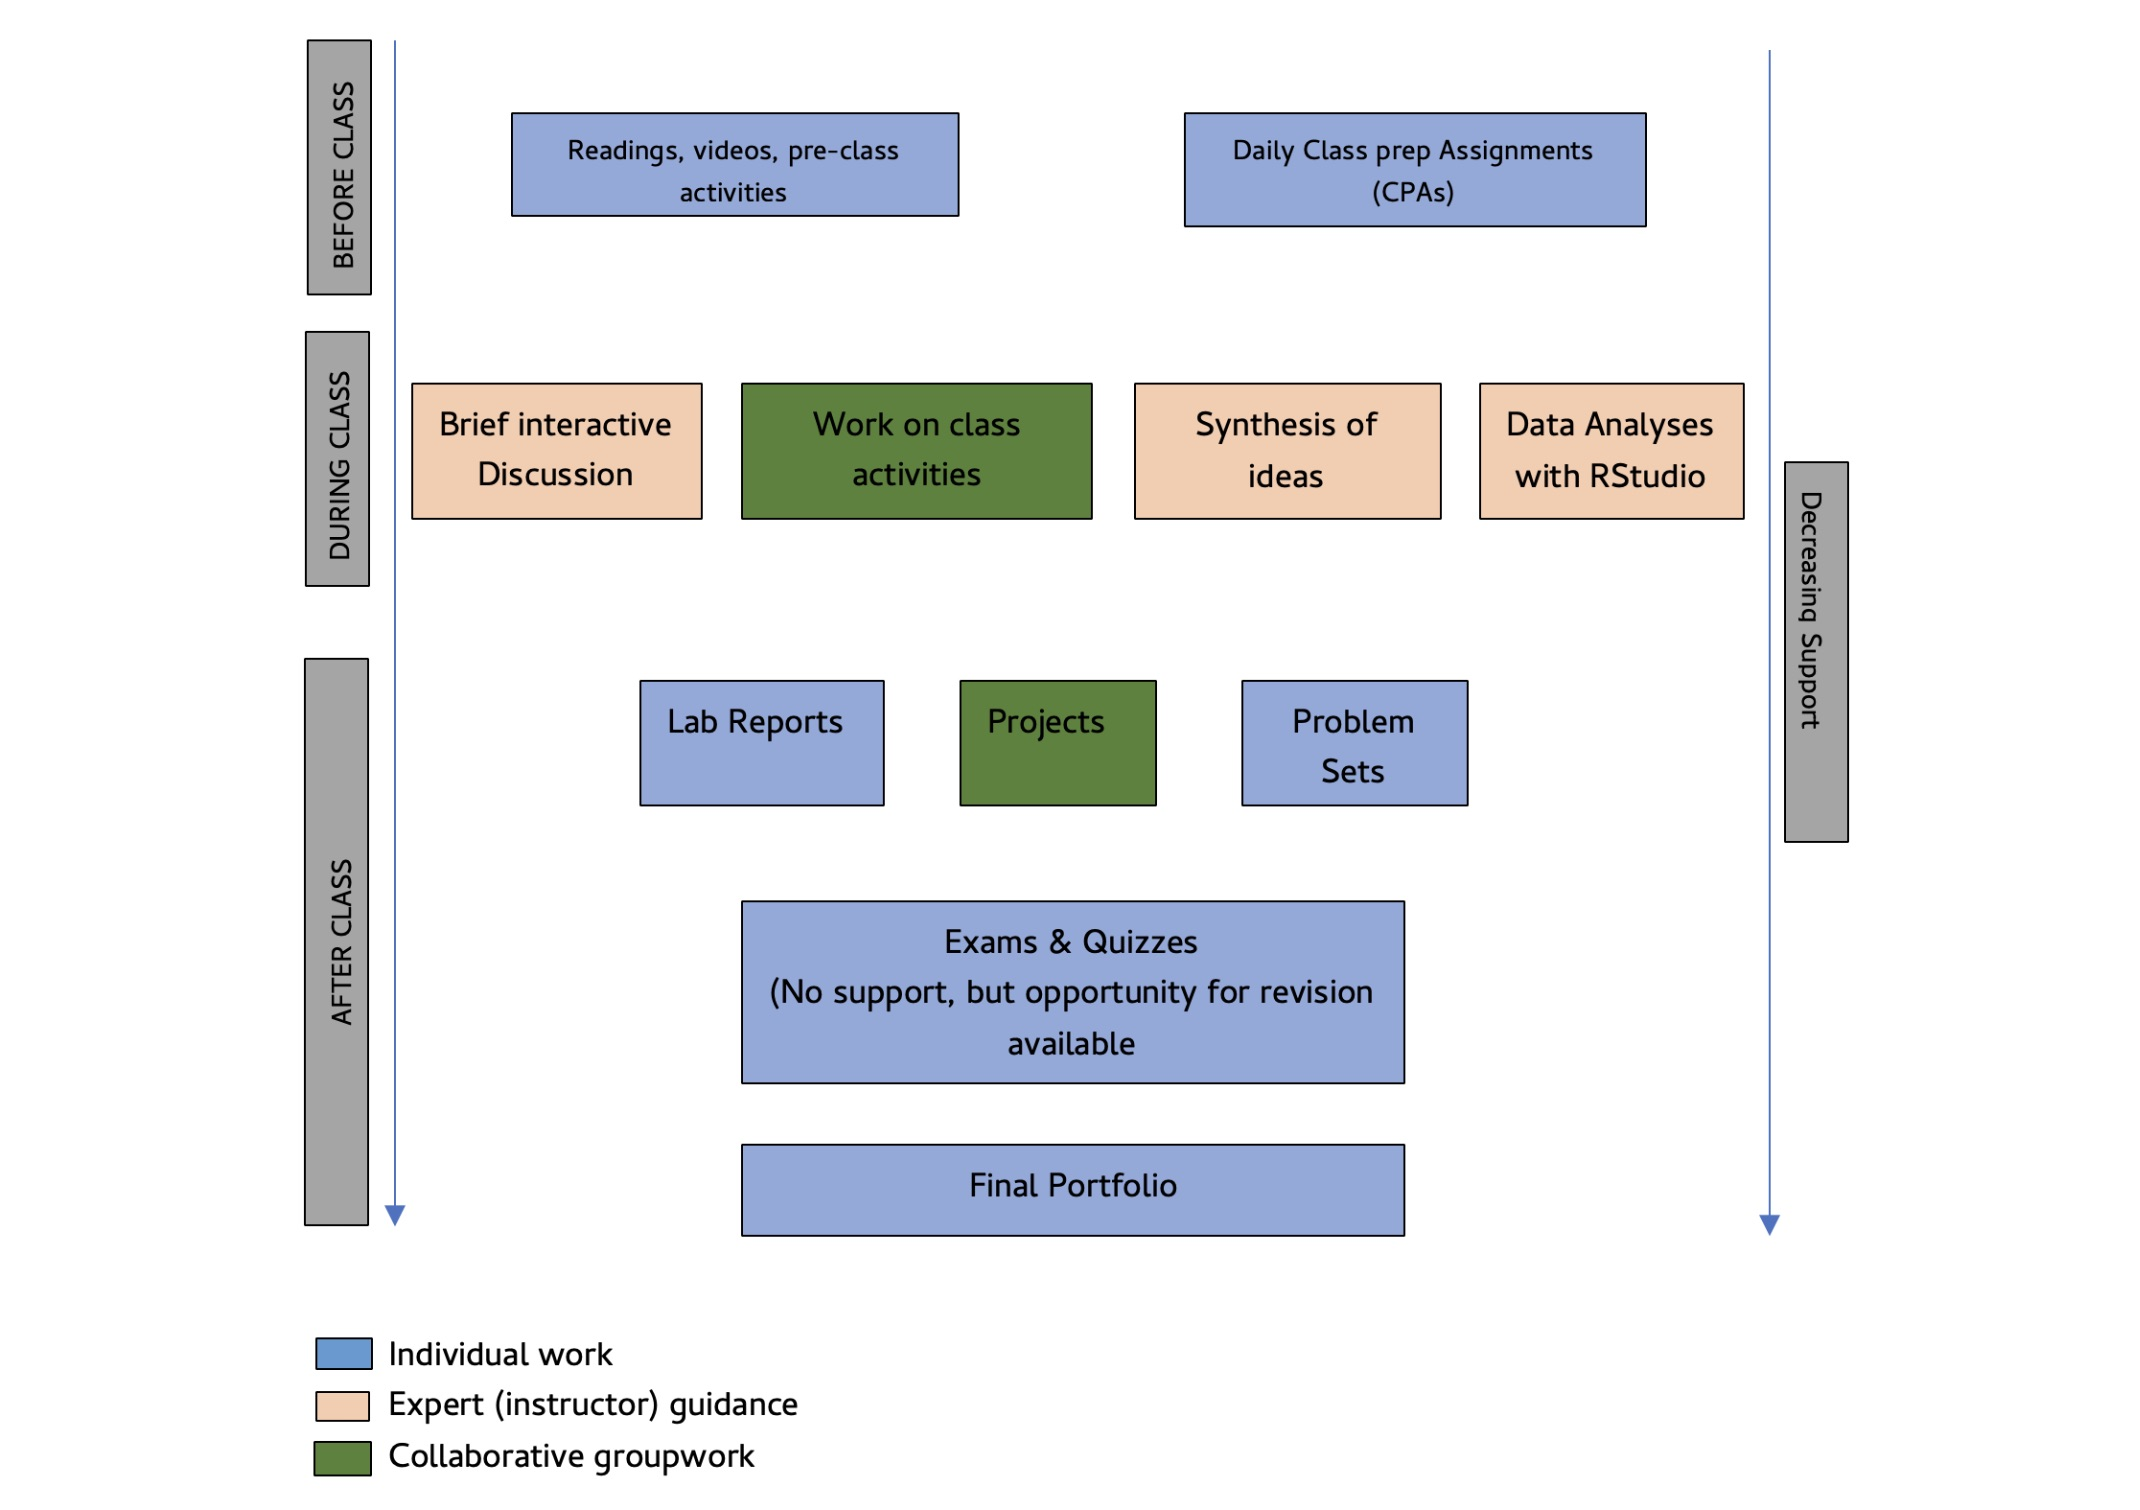
\includegraphics{flip.jpeg}

}

\caption{Flipped Classroom Model}

\end{figure}%

\subsection{Course Resources}\label{course-resources}

\subsubsection{Textbooks}\label{textbooks}

For most of our readings, we shall use the following open-source
textbooks:

\begin{itemize}
\item
  \href{https://openintro-ims.netlify.app/}{Introduction to Modern
  Statistics}, Çetinkaya-Rundel, Hardin. OpenIntro Inc., 2nd Edition,
  2023. Hard copy of the book available
  \href{https://www.amazon.com/dp/1943450277?ref=cm_sw_r_cp_ud_dp_84X75NFMXXJ0N6NTJAEF&ref_=cm_sw_r_cp_ud_dp_84X75NFMXXJ0N6NTJAEF&social_share=cm_sw_r_cp_ud_dp_84X75NFMXXJ0N6NTJAEF&skipTwisterOG=2}{on
  Amazon}.
\item
  \href{https://r4ds.hadley.nz/}{R for Data Science, 2e}, Wickham,
  Çetinkaya-Rundel, Grolemund. O'Reilly, 2nd edition, 2023. Hard copy
  available
  \href{https://www.amazon.com/dp/1492097403?&tag=hadlwick-20}{on
  Amazon}.
\item
  Intermediate Statistics with R by Greenwood, Mark. The book can be
  found freely on
  \href{https://open.umn.edu/opentextbooks/textbooks/1078}{this link}.
\end{itemize}

\subsubsection{Computing:}\label{computing}

\begin{itemize}
\item
  \textbf{R:} We will use R statistical environment with the RStudio
  interface. You'll be using R primarily through a version of RStudio
  accessible on \href{https://posit.cloud/}{posit cloud}. Once you are
  on this page, sign in or click on \textbf{sign up} to create a new
  account in case you don't already have an account.
\item
  \textbf{GitHub Copilot:} GitHub is a web-based platform that allows
  people to store, share, and manage versions of their code. For
  example, a team of programmers working on different parts of a certain
  project may use GitHub for collaboration. We shall use these features
  only sparingly in this course. Copilot, on the other hand, is a
  popular AI-powered tool used for a vast range of purposes including
  code generation. Copilot is a paid service but college students can
  access and use it for free via GitHub (GitHub Copilot). To use GitHub
  copilot and use it within RStudio, there are three steps involved:

  \begin{itemize}
  \item
    \textbf{Step 1:} Sign up for a free GitHub account at
    \href{https://github.com}{GitHub}.
  \item
    \textbf{Step 2:} Sign up for a free GitHub Student Developer Pack
    account at \href{https://education.github.com/pack}{GitHub Student
    Developer Pack}.
  \item
    \textbf{Step 3:} Install the GitHub Copilot extension in RStudio. To
    do this,
  \end{itemize}
\item
  \textbf{Optional:} You may want to have a scientific calculator (one
  that has the ability to compute powers--e.g., \((1.675)^3)\) to use
  when you want to do quick calculations. You may also use online
  calculator tools such as \href{https://www.desmos.com}{desmos}.
\end{itemize}

\subsection{Assessment}\label{assessment}

Your learning will be assessed in a variety of ways including Attendance
and Participation (AP), CPA's, Labs, Problem Sets (PS), Projects, Exams,
and a final Portfolio (takes the place of a final exam). Below are the
details on these components.

\subsubsection{Attendance and Participation
(AP)}\label{attendance-and-participation-ap}

You're expected to attend and participate in class. Consistent
attendance and participation are strong indicators of success in MAT
246. You will be responsible for all course material, announcements,
quizzes, and exams made in class, whether you attended that day's class
or not. I may post the announcements and materials on Canvas and/or send
them out as emails. If you anticipate needing to miss more than four
class sessions, please make an appointment with me to discuss any
restrictions on your availability early in the semester so we can find
ways for you to participate and be successful in the course. Note that
attendance and participation count for 10\% of your overall grade. Your
attendance \& participation grade will be based on the following
metrics:

\begin{itemize}
\tightlist
\item
  Punctuality to class and number of classes attended
\item
  Preparedness for class (you will generally be considered prepared if
  you do the CPAs)
\item
  Level of engagement: Includes working collaboratively with others,
  sharing your thoughts during whole-class discussion, and asking
  questions if necessary.
\item
  Contributing to online collaboration work and discussion forums.
\end{itemize}

For a more detailed rubric on how attendance and participation will be
graded, click on
\href{https://docs.google.com/document/d/1za7s6xJWr5EWzF3-LlHHL8Vyn2_dcfIa/edit}{this
link}.

\subsubsection{Class Preparation Assignments
(CPAs)}\label{class-preparation-assignments-cpas}

CPAs are done \textbf{\emph{prior}} to class. They involve completing
short readings or activities and/or watching videos then answering a few
questions based on the covered material. CPA's are meant to get you
prepared for the material of the week/day so that you can contribute
meaningfully during class discussions. For this reason, deadlines for
CPAs cannot be extended.

\textbf{\emph{Note:}} CPAs will generally be graded for completion and
effort. From time to time, there will be one question on the CPA that
will be graded for accuracy. This question is meant to gauge the extent
to which you understood the material on your own and answers may be
discussed in class.

\subsubsection{Problem sets (PSs)}\label{problem-sets-pss}

Problem sets will be assigned after every three to four weeks or after
completion of a major topic. Unlike the CPAs, the problem sets will be
more open-ended, non-routine, and with a heavy emphasis on real life
applications of the material learned. You are encouraged to consult with
your classmates on the problems but write your own solutions. You may
also come in for Student hours for further help if you need it. Do not
wait until the deadline day to start your problem set.

\subsubsection{Labs}\label{labs}

In labs, you will apply what you've learned in during class to complete
data analysis tasks. You may discuss lab assignments with other
students; however, lab should be completed and submitted individually.
Lab assignments must be typed up using Quarto, all work must be rendered
to pdf format and must be submitted on Canvas by the deadline.

Labs are due at 8 am ET on the indicated due date (generally the Tuesday
after the lab).

The lowest lab grade will be dropped at the end of the semester.

\subsubsection{Quizzes}\label{quizzes}

There will be a short quiz in class almost every week (Fridays). The
quiz will be based mainly on material learned in the CPA and/or
discussed in class for the current or previous week. To do well in these
quizzes, you should complete your CPAs accurately, and attend class. If
there are concepts you have questions about, be sure to ask. All Quizzes
will be closed book and closed notes.

\subsubsection{Projects}\label{projects}

There will be two group projects for this class. For every project, a
short proposal will be due roughly a week after the project is assigned.
Your group will have 10-15 minutes to present your work in class and
then submit the project report a day after presentation. Detailed
information about the project, including a grading rubric, will be
provided.

\subsubsection{Midterm Exams}\label{midterm-exams}

There will be two mid-term exams during the semester. Each midterm exam
will have an in class component and a take-home component.

\begin{itemize}
\item
  \textbf{In-class component:} The in-class component will be
  closed-book and closed notes but calculators will be allowed (not on
  devices like cellphones and computers). You will be allowed to bring a
  2-sided A4 size cheatsheet paper for the in-person component. These
  will be submitted alongside the exam.
\item
  \textbf{The take-home component} May require use of RStudio and will
  be availed in quarto (qmd) format. You will need to type in your
  answers into the quarto document and perform the analyses accordingly.
  You should submit a pdf format but if you face errors rendering due to
  errors in your code, you may submit the .qmd file.
\end{itemize}

The exams will focus on both conceptual understanding of the content and
application through analysis and computational tasks. The content of the
exam will be related to the content in CPAs, problem sets, quizzes,
among others.

\subsubsection{Final Portfolio}\label{final-portfolio}

The final portfolio will consist of the following:

\begin{itemize}
\tightlist
\item
  Revised work (if necessary) on both mid-term exams. Again, you should
  point out the errors on every problem and explain how the revisions
  address the errors.
\item
  Revised work (if necessary) on 2 problem sets with the lowest grades.
  Again, you need to have reflective statements on each problem.
\item
  A reflective essay on your main takeaways from the course and how you
  may implement that knowledge in your field or other real-life
  situations.
\end{itemize}

The final portfolio will be due on the day at time of your final exam
for this course.

\subsubsection{Grading Policy}\label{grading-policy}

Your final letter grade in the course will be weighted by category as
follows:

\begin{longtable}[]{@{}ll@{}}
\toprule\noalign{}
Category & Percentage \\
\midrule\noalign{}
\endhead
\bottomrule\noalign{}
\endlastfoot
Attendance and Participation & \(\ge\) 93 \\
Class Preparation Assignments & 90 - 92.99 \\
Problem Sets & 87 - 89.99 \\
Labs & 83 - 86.99 \\
Quizzes & 80 - 82.99 \\
Midterm Exams & 77 - 79.99 \\
Projects & 73 - 76.99 \\
Final Portfolio & 70 - 72.99 \\
\end{longtable}

The final letter grade will be determined based on the following
thresholds:

\begin{longtable}[]{@{}ll@{}}
\toprule\noalign{}
Letter Grade & Final Course Grade \\
\midrule\noalign{}
\endhead
\bottomrule\noalign{}
\endlastfoot
A & \(\ge\) 93 \\
A- & 90 - 92.99 \\
B+ & 87 - 89.99 \\
B & 83 - 86.99 \\
B- & 80 - 82.99 \\
C+ & 77 - 79.99 \\
C & 73 - 76.99 \\
C- & 70 - 72.99 \\
D+ & 67 - 69.99 \\
D & 63 - 66.99 \\
D- & 60 - 62.99 \\
F & \(<\) 60 \\
\end{longtable}

\subsection{Support}\label{support}

There are various resources available to help you succeed in this
course. Should you feel like you are struggling too much, please don't
hesitate to reach out to me so we can discuss possible ways forward.
Below are some academic support services available to you.

\subsubsection{Open Hours}\label{open-hours}

I will be available during open hours (Mon 12.00 - 01.00 pm) to answer
questions or concerns that you may have in the course. You can simply
walk in during the stated time above. More times may be available but
you will need to check my schedule on
\href{https://calendly.com/jmochogi/20min?month=2024-08}{this link}.
Open hours may be held in-person or virtually depending on circumstances
of the day. Below are the zoom link and passcode for virtual meetings:

\textbf{Zoom Link:}
\href{https://ithaca.zoom.us/j/3364817575?pwd=WlA1S3hJWWZNTTFoWUVaZlA1clhtdz09}{click
here}

\textbf{Passcode:} 850 424

\subsubsection{Math Tutoring Sessions}\label{math-tutoring-sessions}

The mathematics department is committed to the success of all students
enrolled in mathematics courses. Free one-on-one support for your
mathematics coursework is available during select daytime and evening
hours Monday-Friday at the Mathematics Room (Williams Hall 209). The
Mathematics Room is staffed by mathematics faculty and vetted students.
Student tutors offer support to fellow students in courses numbered 200
and below while math faculty offer support in any of the math courses.
For more information and the schedule, please visit the
\href{https://www.ithaca.edu/academics/school-humanities-and-sciences/mathematics/courses-placement-resources/mathematics-support-center}{Math
Support Center}.

\subsubsection{Tutoring and Academic Enrichment
Services}\label{tutoring-and-academic-enrichment-services}

As a supplement to faculty advising and office hours, Tutoring and
Academic Enrichment Services offers exceptional peer resources free of
charge. Learning Coaches provide content-specific peer tutoring in a
variety of courses. Peer Success Coaches mentor students who wish to
develop collegiate-level academic and social engagement skills. To
access these courses and for more information, please visit the
\href{https://www.ithaca.edu/tutoring-services}{Center for Student
Success}.

\subsubsection{Writing Center}\label{writing-center}

The Writing Center aims to help students from all disciplines,
backgrounds, and experiences to develop greater independence as writers.
We are committed to helping students see writing as central to critical
and creative thinking. The physical location in Smiddy 107 will not be
open to clients. For more information and scheduling appointments please
visit the \href{https://ithaca.mywconline.com}{writing center website}.

\subsection{Tips for Success}\label{tips-for-success}

Here are a few basic suggestions for how to succeed in this course:

\subsubsection{Keep up with Homework}\label{keep-up-with-homework}

It is absolutely essential that you understand how to solve the assigned
homework problems/exercises and, more importantly, how and why the
skills and techniques presented in the course are used in solving the
problems/exercises. I suggest that you begin working on the how as soon
as possible. Do not pile your haw or work near the deadline. The
advantage of getting the homework done on time is that you will get
timely feedback that will help you understand the material better and
hence do well in other assessment categories such as exams.

\subsubsection{Attend Class}\label{attend-class}

As noted earlier, attendance is a critical part of your success in this
course. You should try to attend every class because it is during class
time that we will delve deeper into the course material and practice
with applications.

\subsubsection{Stay Caught Up}\label{stay-caught-up}

Most concepts in this course build on each other cumulatively and you
need to stay on top of the material at every stage. If you are having
difficulty, don't expect that the problem will take care of itself and
disappear later. Contact me immediately and discuss the problem.

\subsubsection{Collaborate with Peers}\label{collaborate-with-peers}

Many students benefit from sharing their work with others or by having
their work questioned by their peers. You should attempt homework
problems ahead of time by yourself and then note down any
difficulties/questions that you can discuss with your peers. Even if you
have no difficulties, you may still learn different and perhaps more
efficient ways of solving the same problem during collaborative work.
Below are some of the ways through which you can do this: -
\textbf{Canvas Discussion Forums \& One Note Collaboration Space} - You
can post questions and answer others' questions here. I encourage you to
scan hand-written work (if necessary) and upload it alongside your
question so people can see how you are thinking.

\begin{itemize}
\tightlist
\item
  \textbf{Zoom sessions} -- If you cannot meet in person, you can
  initiate Zoom sessions for collaborating. Zoom whiteboards are
  available to write on or you may simply have discussions. You can
  record these for later playback. If you want to invite me to your Zoom
  session, please send me an email with the link ahead of time and I
  will let you know if I am available to join.
\end{itemize}

\subsection{College-wide Policies}\label{college-wide-policies}

\subsubsection{Student Accessibility
Services}\label{student-accessibility-services}

In compliance with Section 504 of the Rehabilitation Act of 1973 and the
Americans with Disabilities Act, reasonable accommodation will be
provided to students with documented disabilities on a case-by-case
basis. Students must register with
\hyperref[student-accessibility-services]{Student Accessibility
Services} (https://www.ithaca.edu/student-accessibility-services) and
provide appropriate documentation to Ithaca College before any academic
adjustment will be provided.

\subsubsection{Mental Health statement}\label{mental-health-statement}

Diminished mental health, including significant stress, mood changes,
excessive worry, or problems with eating and/or sleeping can interfere
with optimal academic performance. The source of symptoms might be
related to your course work; if so, please speak with me. However,
problems with relationships, family worries, loss, or a personal
struggle or crisis can also contribute to decreased academic
performance. Ithaca College provides no-additional-cost mental health
services through the Center for Counseling and Psychological Services
(CAPS) to help you man- age personal challenges that threaten your
personal or academic well-being. In the event that I suspect you need
additional support, expect that I will express to you my concerns and
the rea- sons for them. It is not my intent to know the details of what
might be troubling you, but simply to let you know I am concerned and
that help (e.g., CAPS, ICare, Health Center, Chaplains, etc\ldots), if
needed, is available. Remember, getting help is a smart and courageous
thing to do.

\subsubsection{Academic Integrity}\label{academic-integrity}

The College is an academic community, which values academic integrity
and takes seriously its responsibility for upholding academic honesty.
All members of the academic community have an obligation to uphold high
intellectual and ethical standards. All forms of dishonesty including
cheating and plagiarism are unacceptable. Failure to appropriately cite
material used in a paper is plagiarism. The minimum penalty for cheating
or plagiarism is a zero for the test or paper in question. Referral to
college judiciaries is also possible. For more information on academic
integrity and academic dishonesty, please refer to the
\href{https://www.ithaca.edu/student-affairs-and-campus-life/student-handbook}{Student
Handbook}, the College Catalog and the
\href{https://www.ithaca.edu/policy-manual/volume-vii-students/71-general-student-policies/712-student-conduct-code}{Code
of Student Conduct} and Related Policies or ask your instructor.

\subsubsection{Title IX}\label{title-ix}

At Ithaca College, we believe that every individual has the right to be
treated with respect and dignity and we support the creation and
maintenance of a safe and positive living and learning environment.
Students who experience sexual violence (including dating violence,
stalking and sexual assault), sexual harassment, or discrimination based
on gender or sexual identity) are encouraged to report their experience
to the Title IX Coordinator, lkoenig@ithaca.edu to explore formal and
informal reporting options, and explore the support and resources
available. The Title IX Coordinator will work with you to determine the
best way to proceed and enhance the safety of our community. For more
information go to: \url{https://www.ithaca.edu/share}.

Information shared in class assignments, class discussions, and at
public events do not constitute an official disclosure, and faculty and
staff do not have to report these to the Title IX Coordinator. Faculty
and staff should be sure that access to campus and community resources
related to sexual misconduct are available to students in the case these
subjects do arise. Any other disclosure to faculty and staff can be
reported to the Title IX Coordinator.

\subsubsection{Academic Advising Center}\label{academic-advising-center}

As a complement to a student's faculty advisor(s), the professional
academic advisors in the AAC are available to help students discuss the
outcomes of academic decisions, explore academic choices, and to examine
the consequences of changing a major or adding a minor. Students(first
year through senior) from any major can make an appointment by calling
607-274-1001 or emailing
\href{mailto:advisingcenter@ithaca.edu}{\nolinkurl{advisingcenter@ithaca.edu}}.

\subsubsection{Diversity and Inclusion}\label{diversity-and-inclusion}

Ithaca College values diversity because it enriches our community and
the myriad experiences that characterize an Ithaca College education.
Diversity encompasses multiple dimensions, including but not limited to
race, culture, nationality, ethnicity, religion, ideas, beliefs,
geographic origin, class, sexual orientation, gender, gender identity
and expression, disability, and age. We are dedicated to addressing
current and past injustices and promoting excellence and equity. Ithaca
College continually strives to build an inclusive and welcoming
community of individuals with diverse talents and skills from a
multitude of backgrounds who are committed to civility, mutual respect,
social justice, and the free and open exchange of ideas. We commit
ourselves to change, growth, and actions that embrace diversity as an
integral part of the educational experience and of the community we
create.Please learn more about Ithaca College's commitment to diversity,
equity and inclusion:
\url{https://www.ithaca.edu/diversity-and-inclusion/diversity-statement}.

\subsection{Course policies}\label{course-policies}

\subsubsection{Academic honesty}\label{academic-honesty}

The point is very simple - {you should not cheat.} You should not
present ``someone'' else's work as your own.

Abide by the following guidelines:

\begin{itemize}
\item
  \textbf{Collaboration:}

  \begin{itemize}
  \tightlist
  \item
    Work that is not assigned as a collaborative assignment should not
    be completed collaboratively. This does not mean you should not seek
    support from peers. If you seek help from your peers, be sure that
    you write your own solutions, otherwise the work will be similar and
    flagged for cheating. Submitting similar work will be considered a
    violation of the academic integrity policy by all students involved.
  \item
    For team assignments, you may collaborate freely within your team.
    Each group will submit one document contained agreed upon responses.
    No multiple file submissions.\\
  \item
    On individual assignments you may not directly share work with
    another student in this class, and on team assignments you may not
    directly share work with another team in this class.
  \end{itemize}
\item
  \textbf{Online resources:} In this century, the internet is a go to
  place for many things. While much of the information on the internet
  is useful, I expect that you will use it responsibly. The course
  policy is that you may use online resources (e.g.,
  \href{https://stackoverflow.com/}{StackOverflow},
  \href{https://www.wolframalpha.com/}{Wolfram Alpha}, etc.) but you
  must explicitly cite where you obtained any solutions you directly use
  (or use as inspiration).
\item
  \textbf{Use of generative artificial intelligence (AI)}: Generative AI
  tools such as ChatGPT should be treated as other online resources.
  There are two guiding principles that govern how you can use AI in
  this course:

  \begin{itemize}
  \item
    \emph{Cognitive dimension:} Using AI tools should make you more
    efficient and productive rather than hampering your ability to think
    clearly and critically.
  \item
    \emph{Ethical dimension:} Students using AI should be transparent
    about their use and make sure it aligns with academic integrity. You
    are ultimately responsible for the work you turn in; it should
    reflect your understanding of the course content. AI is an integral
    part of this course and we will practice using generative AI tools
    responsibly without losing sight of the learning objectives.
  \item
    \textbf{✅ AI tools for code:} We will use GitHub Copilot for code
    generation in this course. However, we will only start using this
    tool after you have gained a basic understanding of the coding and
    syntax. While coding uses highly specified formats and even minor
    errors can cause problems, using github copilot can be thought of as
    ``coding in English''. You will just need to prompt the tool
    effectively. You should also examine the code output as much as
    possible. One way to do this is to look at the output (if available)
    and work backwards. More details on this to follow.
  \end{itemize}

  You may use
  \href{https://guides.lib.monash.edu/c.php?g=219786&p=6972087}{these
  guidelines} for citing AI-generated content.

  \begin{itemize}
  \tightlist
  \item
    \textbf{❌ AI tools for narrative:} You may not use generative AI
    tools such as ChatGPT to write narrative on assignments.
    Interpretation of software output, writing up the project report,
    among others should be written by a human (YOU). If you want to use
    these tools to check your grammar, you should feel free to do so but
    be sure to disclose and cite it accordingly.
  \end{itemize}
\end{itemize}

If you are unsure if the use of a particular resource complies with the
academic honesty policy, please contact your instructor.

\subsubsection{Late work}\label{late-work}

The due date \& time for all assignments will be posted on Canvas and/or
emailed out and/or announced in class. To enable me to prepare for class
meetings and give you feedback, {I will not accept late work} except
under extreme circumstances. If you know that you won't be able to turn
in an assignment on time, reach out to me in writing (email) at least
one day before the due date to discuss your options. Note that there
will be {no extensions on CPA's}.

\subsubsection{Mobile devices \& Other
Technologies}\label{mobile-devices-other-technologies}

This class allows use of technology devices (e.g., computers, tablets,
etc.) only for purposes of the course. Such purpose involves data
analysis, writing reports, completing OneNote collaborative activities,
among others. However, there will be moments (e.g., brief interactive
discussion, completing paper activities,) when I require that students
put away (or turn off) their technology devices. Use of these devices
for purposes other than the one for the course is prohibited. Research
on this matter shows that it distracts you as well as other students in
class. Two violations per week will result in a 0 score on the next
attendance and participation grade. Persistent violation may necessitate
further action to prevent you from distracting other students.

\subsubsection{Groups}\label{groups}

This class will mostly run through small group work. You will be
randomly assigned to a group at the start of the semester. About midway
into the semester, I will switch people around based partly on my
professional judgement. I will allow you to suggest members you would
like to work with but there are no guarantees that you will get grouped
with all members of your choice. I generally seek to have mixed ability
groups and to ensure that everyone has a chance to work with different
people.

\begin{tcolorbox}[enhanced jigsaw, colframe=quarto-callout-note-color-frame, rightrule=.15mm, leftrule=.75mm, coltitle=black, colback=white, title=\textcolor{quarto-callout-note-color}{\faInfo}\hspace{0.5em}{Click here for syllabus bounty!}, left=2mm, colbacktitle=quarto-callout-note-color!10!white, opacitybacktitle=0.6, toprule=.15mm, arc=.35mm, bottomrule=.15mm, titlerule=0mm, toptitle=1mm, breakable, bottomtitle=1mm, opacityback=0]

If you've read this far in the syllabus, please email me a picture of
your favorite scene in Ithaca or its environs if you have one. If not,
just describe the place. I will include you on my special list of most
serious students.

\end{tcolorbox}

\subsection{Important dates}\label{important-dates}

\begin{itemize}
\item
  \textbf{Aug 26:} Classes begin, Request S/D/F Option
\item
  \textbf{Sep 01:} Last day to Drop/add a course
\item
  \textbf{Sep 02:} No classes (Labor Day)
\item
  \textbf{Sep 13:} Last day to request S/D/F Option
\item
  \textbf{Sep 27:} Last Day to Withdraw with ``W'', Revoke S/D/F Option
\item
  \textbf{Oct 08:} Project 1 Presentations
\item
  \textbf{Oct 09:} Exam 1 (in-class)
\item
  \textbf{Oct 10:} Exam 1 take-home due
\item
  \textbf{Oct 13:} Midterm grades available online
\item
  \textbf{Oct 17-18:} Fall break - No classes
\item
  \textbf{Nov 01:} Last Day to Withdraw with ``W''
\item
  \textbf{Nov 15:} Exam 2 (in-class)
\item
  \textbf{Nov 16:} Exam 2 take-home due
\item
  \textbf{Nov 23-Dec 1:} Thanksgiving Break - No classes
\item
  \textbf{Nov 27-29:} Project 2 presentations
\item
  \textbf{Dec 11:} Last day of classes
\item
  \textbf{Dec 11:} Final portfolio due
\end{itemize}

Assignment deadlines are listed on the course schedule and in Canvas.
Class ends on April 24, there is no final exam.

For more important dates, see the full
\href{https://www.ithaca.edu/academics/registrar/academic-calendars}{Ithaca
College Calendar}.



\end{document}
